\FloatBarrier
\section{NEAREST} \label{sec:NEAREST}
While FMM algorithms allow for the computation of large N-body problems to be computed, it is complex and time consuming to implement efficiently. A better way to reduce computation time and memory resources is to reduce the overall size of the system. Based on analysis done in by Gallagher, Choudhuri And Smith \cite{Gallagher2019SharpEquation} the total error for the method of regularised stokeslets is found to be $\mathcal{O}(\epsilon) + \mathcal{O}(h) + \mathcal{O}(h^2\epsilon^{-1}) + \mathcal{O}(P\epsilon^{-1/P} h^{1-P})$ for $P>3$. In order to reduce the overall error, a reduction in $\epsilon$ is required such that the regularisation error term $\mathcal{O}(\epsilon)$ decreases, however doing this necessitates the reduction in $h$ from the $\mathcal{O}(h^2\epsilon^{-1})$ term, the average quadrature spacing, to keep the discretisation error at a similar size. In order to still fully cover our boundary, the number of quadrature points used in the calculation must therefore be increased, which will increase the computations needed to both perform the direct vector-matrix product or the matrix inversion required for resistance problems. 

Alternative methods of solving Stokes flow such as the Boundary Element Method (BEM) for Stokes flow developed by Phan-Thien et al \cite{Tran-Cong1987APropulsion} allow for solutions to singular systems with highly refined meshes. The BEM method allows for the decoupling of the quadrature and traction discretisation allowing for the singular stokeslet kernel to be evaluated by the most appropriate means without affecting the overall number of degrees of freedom. While these ideas have been applied to regularised stokeslet systems by Schuech and Smith\cite{Smith2009AFlow,SchuechMotilePareto-optimal} and have been shown to perform with 3 orders of magnitude less processing time and memory when compared to the Nyström method, but they still require a connected mesh to be generated on the boundary. 

The NEAREST method proposed by Smith \cite{Smith2018AEquation} aims to again decouple the quadrature and traction discretisation while still preserving the simplicity of the low order quadrature rule of the Nyström. Due to the use of low order quadrature rules the NEAREST method does not require the generation of a connected mesh making it significantly easier to implement compared to the Boundary element method. To decouple the quadrature and traction discretisation the NEAREST method employs two discretisations of the surface $\partial D$, one coarse and one fine denoted by $\{\bm{x}_1, \dots, \bm{x}_n\}$ and $\{\bm{X}_1, \dots, \bm{X}_Q\}$ respectively. The coarser discretisation captures the variation in the traction over the surface and the finer discretisation needs to have sufficient resolution to capture the rapidly varying stokelet kernel $S^\epsilon$. For this reason we will assume that the number of points in the fine set $Q$ to be larger than that in the coarse set $N$. The boundary integral method requires that we know the force at the quadrature set which, by definition, is not calculated for all points $\{\bm{X}_q\}$, however, as the force varies slowly over the surface, the NEAREST method approximates the force at the fine quadrature $\bm{f}(\bm{X}_q)dS(\bm{X}_q)$ points by the force at the nearest point in the coarse force quadrature set $\bm{f}\left(\bm{x}(\mathcal{N}(q)\right) d S(\bm{x}\mathcal{N}(q))$, where 
\begin{equation}
\label{eq:NEARESTmap}
    \mathcal{N}(q) := \underset{n=1, \ldots, N}{\operatorname{argmin}}|\boldsymbol{x}_n-\boldsymbol{X}_q|
\end{equation}

\subsection{Derivation of the NEAREST discretisation}
The formulation of the NEAREST discretisation takes the standard form of the boundary integral equation (eq.~\ref{eq:BIE}) and replaces the force and surface metric at a point $\bm{y}$ with the mapping of $\bm{y}$ to its closest force point.

This allows us to define \cref{eq:BIE} as 
\begin{equation}
\begin{aligned}
\label{eq:BIENearest1}
        u_i(\bm{y}) &= \frac{1}{8 \pi \mu} \int_{\partial D} S_{i j}^{\epsilon}\left(\bm{y}, \bm{X}_q\right) f_{j}(\bm{X}_q) d S(\bm{X}_q) \\
        &= \frac{1}{8 \pi \mu} \int_{\partial D} S_{i j}^{\epsilon}\left(\bm{y}, \bm{X}_q\right) f_{j}(\mathcal{N}(q)) d S(\mathcal{N}(q)) \\
        & = \frac{1}{8 \pi \mu} \sum_{q=1}^Q S_{i j}^{\epsilon}\left(\bm{y}, \bm{X}_q\right){f_{j}}[\mathcal{N}(q)]A[\mathcal{N}(q)]
\end{aligned}
\end{equation}
where the final line is the discretisation of the integral with the fine quadrature points. The Nearest operator $\mathcal{N}(q)$ is written as a sparse matrix $Q \times N$ operator defined by
\begin{equation}
\label{eq:NNMatrix}
    \nu [q, \hat{n}]= \begin{cases} 1 & \text { if } \hat{n}=\underset{n=1, \ldots, N}{\operatorname{argmin}}|x_n-X_q| , \\ 0 & \text { otherwise. }\end{cases}
\end{equation}
This provides a direct mapping for each point from our fine quadrature set to the coarse force set. When considering large quadrature sets, we can find cases where a fine quadrature point is equidistant to two or more force points. Under the current form of $\nu [q, \hat{n}]$ the quadrature point is mapped to the first force point in the set. This means that the same set of force and quadrature points can have different results depending on how both sets are arranged. If we instead split the quadrature point contribution evenly between all equidistant force points, we can eliminate this problem. This can be implemented by replacing the first condition when $\hat{n}=\underset{n=1, \ldots, N}{\operatorname{argmin}}|x_n-X_q|$ with $1/k$ where $k$ is the number of points in $\{x_n\}$ which are equidistant to $\{X_q\}$. This allows a fine point to be mapped to multiple coarse points if they are equidistant, with its contribution evenly distributed between them. The sparse matrix form of $\mathcal{N}(q)$ allows us to express \cref{eq:BIENearest1} as 
\begin{equation}
    u_i(\bm{y}) = \frac{1}{8 \pi \mu} \sum_{n=1}^q  f_{j}(\bm{x}_n) A_n \sum_{q=1}^{Q}S_{i j}^{\epsilon}\left(\bm{y}, \bm{X}_q\right) \nu[q,n] 
\end{equation}
As we considered in the direct product \cref{eq:matrixvectorproduct}, we can calculate the velocity at a set of collocation points $\{x_n\}$ with $n=1,\dots,N$ as a matrix-vector product. If we write $\underline{U}$ and $\underline{F}$ as before, the stokeslet matrix $A$ now takes the form of a $3N \times 3Q$ matrix. The nearest neighbour matrix $\nu [q, \hat{n}]$ can be used by taking the Kronecker product of $\nu$ with the $3 \times 3$ identity matrix ($\Pi = \nu \otimes \mathds{1}_{3}$) to map each axis at every point. This allows us to form the system
\begin{equation}
    \underline{U} = A \cdot \Pi \cdot \underline{F}.
\end{equation}
The NEAREST method allows for both the forward matrix product to compute the velocity of the fluid as well as solving the resistance problem through $\underline{F} = (A \cdot \Pi)^{-1} \underline{U}$. The NEAREST method is not directly aimed at competing directly with BEM methods but in practice it does offer an easier mesh-free adaptation to the standard Nyström method, which allows for the computation of larger-scale systems, than that of the standard direct product.

By introducing the second discretisation we have now changed the error estimations for the method, we keep the regularisation error of $\mathcal{O}(\epsilon)$ and traction discretisation error $\mathcal{O}(h_f)$. The quadrature error now depends on whether the traction points are contained (within distance $O(\epsilon)$ or closer) in the quadrature set. We introduce the distances $h_q$ and $h_f$ to be the length scales associated with the quadrature and force discretisation respectively. In the contained case we obtain a quadrature error of $\mathcal{O}(\epsilon^{-1}h^2_q) + \mathcal{O}(P\epsilon^{-1/P}h^{1-1/P}_q)$ for all integer $P>3$ and for the disjoint case the error decouples from $\epsilon$ to be $\mathcal{O}(h^3_q\delta^{2}) + \mathcal{O}(Ph^{1-2/P}_q)$ where $\delta$ is the closest distance between quadrature and traction points \cite{Gallagher2019SharpEquation}.

\subsection{Comparison of NEAREST to Nyström method}
In order to illustrate the benefits of using the NEAREST discretisation, we will consider the resistance problem in \cref{sec:resistance} for a sphere of unit radius for which we have an exact solution (eq.~\ref{eq:sphereres}) to compare our method with. The construction of the Grand resistance matrix involves solving $6$ resistance problems, three for the unit translations velocities along each axis and three for the unit angular velocities. From each resistance problem we find the total force and moment on the body by summing over all forces of the sphere. This gives us an approximation to $\mathcal{R}$, $\mathcal{R}^\epsilon$. The relative error between the two solutions is then found by 
\begin{equation}
    \text { relative error }=\frac{\left\lVert \mathcal{R}-\mathcal{R}^{\epsilon}\right\rVert_{2}}{\lvert\mathcal{R}\rVert_{2}} \text {, }
    \label{eq:RelativeError}
\end{equation}
where ${\lvert\mathcal{R}\rVert_{2}}$ is the 2-norm of the matrix ($\lvert\mathcal{R}\rVert_{2}=\sup_{x \neq 0}\lvert\mathcal{R}x\rVert_{2} /\lvert x\rVert_{2}$).
The sphere is then discretised into two quadrature sets. A coarse force set with an approximate spacing of $h$ and a fine quadrature set with a spacing of $h/4$. Figure \ref{fig:NEARESTCOMP} illustrates the relative error for the range of quadrature spacing and epsilon. 

\begin{figure}
    \centering
    \subfloat[\label{fig:NYSTROM}]{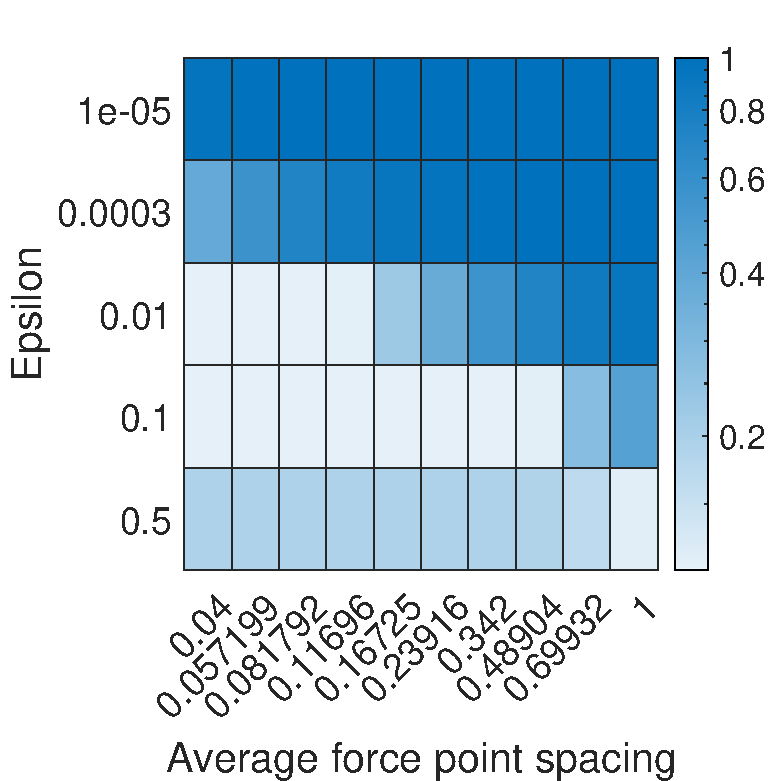
\includegraphics[width=0.45\textwidth]{Images/NEAREST/Nystrom.pdf}}
    \subfloat[\label{fig:DIS}]{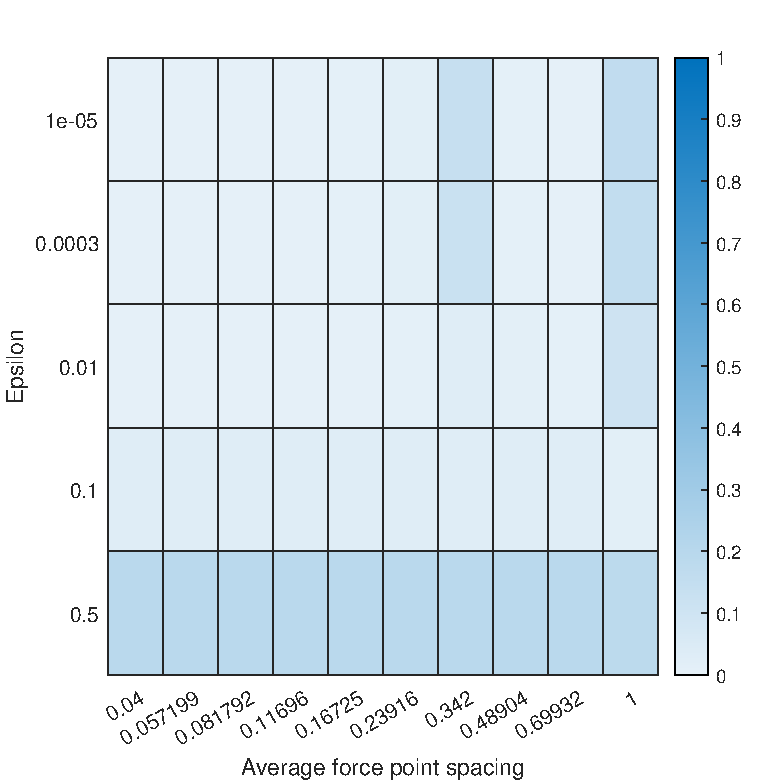
\includegraphics[width=0.45\textwidth]{Images/NEAREST/Disjoint.pdf}}\\
    \subfloat[\label{fig:JOIN}]{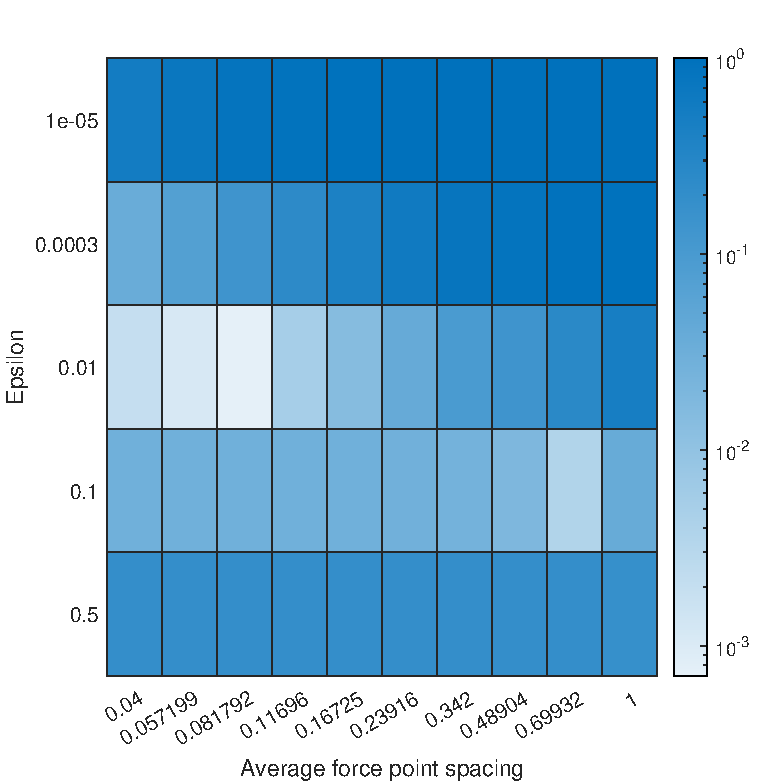
\includegraphics[width=0.45\textwidth]{Images/NEAREST/Intersecting.pdf}}
    \caption[The relative error in calculating the grand resistance matrix for the unit sphere using Nyström and NEAREST.]{The relative error in calculating the grand resistance matrix for the unit sphere using Nyström and NEAREST. (i) Relative error in Grand Residence matrix for the Nyström method. (ii) Relative error in Grand Residence matrix for the disjoint NEAREST method. (iii) Relative error in Grand Residence matrix for the contained NEAREST method.}
    \label{fig:NEARESTCOMP}
\end{figure}

While both the NEAREST and Nyström method benefit from a finer quadrature set all computations were achieved in a similar time with at worst NEAREST taking 29\% longer in computation at the finest discretisation when computed on (M2) using gpuArrays from MATLABs Parallel Computing Toolbox \cite{Gallagher2020} and all methods computing in under 370 seconds. The Nyström method achieves under 2\% errors for several pairs of $h$ and $\epsilon$ but with results quickly diverging as the quadrature error is decreased. We see a similar pattern for the contained NEAREST method where the fine quadrature set includes both the refined quadrature points as well as the coarse force points. This is to be expected as the contained NEAREST method retains the dependence on $\epsilon$ from the NEAREST method but improves upon the error expected for a given $h$. We do notice a large difference in the disjoint NEAREST method where the dependence on epsilon has been removed almost entirely with all pairs giving errors of less than 20\% and the smallest values of $h$ giving errors of less than 0.05\%. 
